% Definition des grundsätzlichen Aufbaus
\documentclass[11pt,a4paper]{article}
\usepackage[utf8]{inputenc}
\usepackage[german]{babel}
\usepackage[a4paper,top=30mm,bottom=20mm,left=40mm,right=25mm]{geometry}
\usepackage[onehalfspacing]{setspace}
\usepackage{lmodern}

% Symbole für mathematische Formeln
\usepackage{amsmath}
\usepackage{amsfonts}
\usepackage{amssymb}

% Tabellen und Grafiken
\usepackage{booktabs}
\usepackage{float}
\usepackage{graphicx}
\usepackage{hyperref}

% Sonstige Anpassungen
\usepackage[printonlyused]{acronym}
\setlength\belowcaptionskip{10pt}

% Literaturverzeichnis
\usepackage{csquotes}
\usepackage[style=apa, backend=biber]{biblatex}
\addbibresource{references.bib}

% Beginn des Dokuments
\begin{document}

% Titelseite
\setcounter{page}{0} % nummeriert Titelseite in PDF mit Seite 0
	\begin{titlepage}
		\begin{center}
			{\LARGE\scshape Universität Hamburg}\\*[5mm]
      		{\normalsize Fakultät für Betriebswirtschaft\\
			Institut für Logistik, Transport und Verkehr}\\*[3cm]
      		{\Large\scshape Bachelor/Masterarbeit/Seminararbeit}\\*[12mm]
      		{\bfseries\Large\scshape Titel der Bachelor/Masterarbeit}\\*[12mm] % hier Titel einfügen #############
      		{\rmfamily Freie wissenschaftliche Arbeit\\
           	zur Erlangung des Grades "`Bachelor/Master of Science"'\\
           	im Studiengang \ldots} \\*[12mm]
      		{\normalsize\rmfamily Hamburg, \ldots} % hier Datum einfügen #############
		\end{center}
		\vspace{8cm}
		\begin{tabbing}
			Fachsemester: \= \hspace{70mm}\= \kill
 			eingereicht von: \>\> betreut von: \\*[2mm]
      		\textbf{NAME, VORNAME} \>\>  Prof. Dr. Knut Haase\\*[2mm] % hier Name einfügen #############
      		Matrikel-Nr.: \> XXXXXXX \>  \\*[2mm] % hier Matrikelnummer und Betreuer einfügen #############
      		Fachsemester: \> X \\*[2mm] % hier Fachsemester einfügen #############
      		E-Mail: vorname.name@studium.uni-hamburg.de % hier E-Mail-Adresse einfügen #############
		\end{tabbing}
  \end{titlepage}

% Inhaltsverzeichnis
\newpage
\pagenumbering{Roman}
\tableofcontents

% Abbildungsverzeichnis
\newpage
\addcontentsline{toc}{section}{Abbildungsverzeichnis}
\listoffigures

% Tabellenverzeichnis
\newpage
\addcontentsline{toc}{section}{Tabellenverzeichnis}
\listoftables

% Abkürzungsverzeichnis
\newpage
\addcontentsline{toc}{section}{Abkürzungsverzeichnis}
\section*{Abkürzungsverzeichnis}
\begin{acronym}[Bash]
	\acro{meA}{meine eigene Abkürzung}
\end{acronym}

% Symbolverzeichnis
\newpage
\addcontentsline{toc}{section}{Symbolverzeichnis}
\section*{Symbolverzeichnis}
\begin{tabular}{p{0.08\textwidth} p{0.92\textwidth}}
	$d_i$ &	Kapazität der Maschine $i\in \mathcal{I}$\\
	$\mathcal{I}$ & Menge der Maschinen\\
	$\mathcal{J}$ & Menge der Produkte\\
        $\mathcal{K}$ & Menge der Menschen\\
	$Z$ & Symbole sind alphabetisch sortiert
\end{tabular}

\newpage
\pagenumbering{arabic}

% Inhalt
\section{Einführung}
Die erste Anwendung \ac{meA} wird ausgeschrieben.
Anschließend wird \ac{meA} abgekürzt.
Die Abbildung \ref{fig:food} zeigt den Streckenverlauf der Mekka Metro in Saudi Arabien.

\begin{figure}[H]
	\centering
	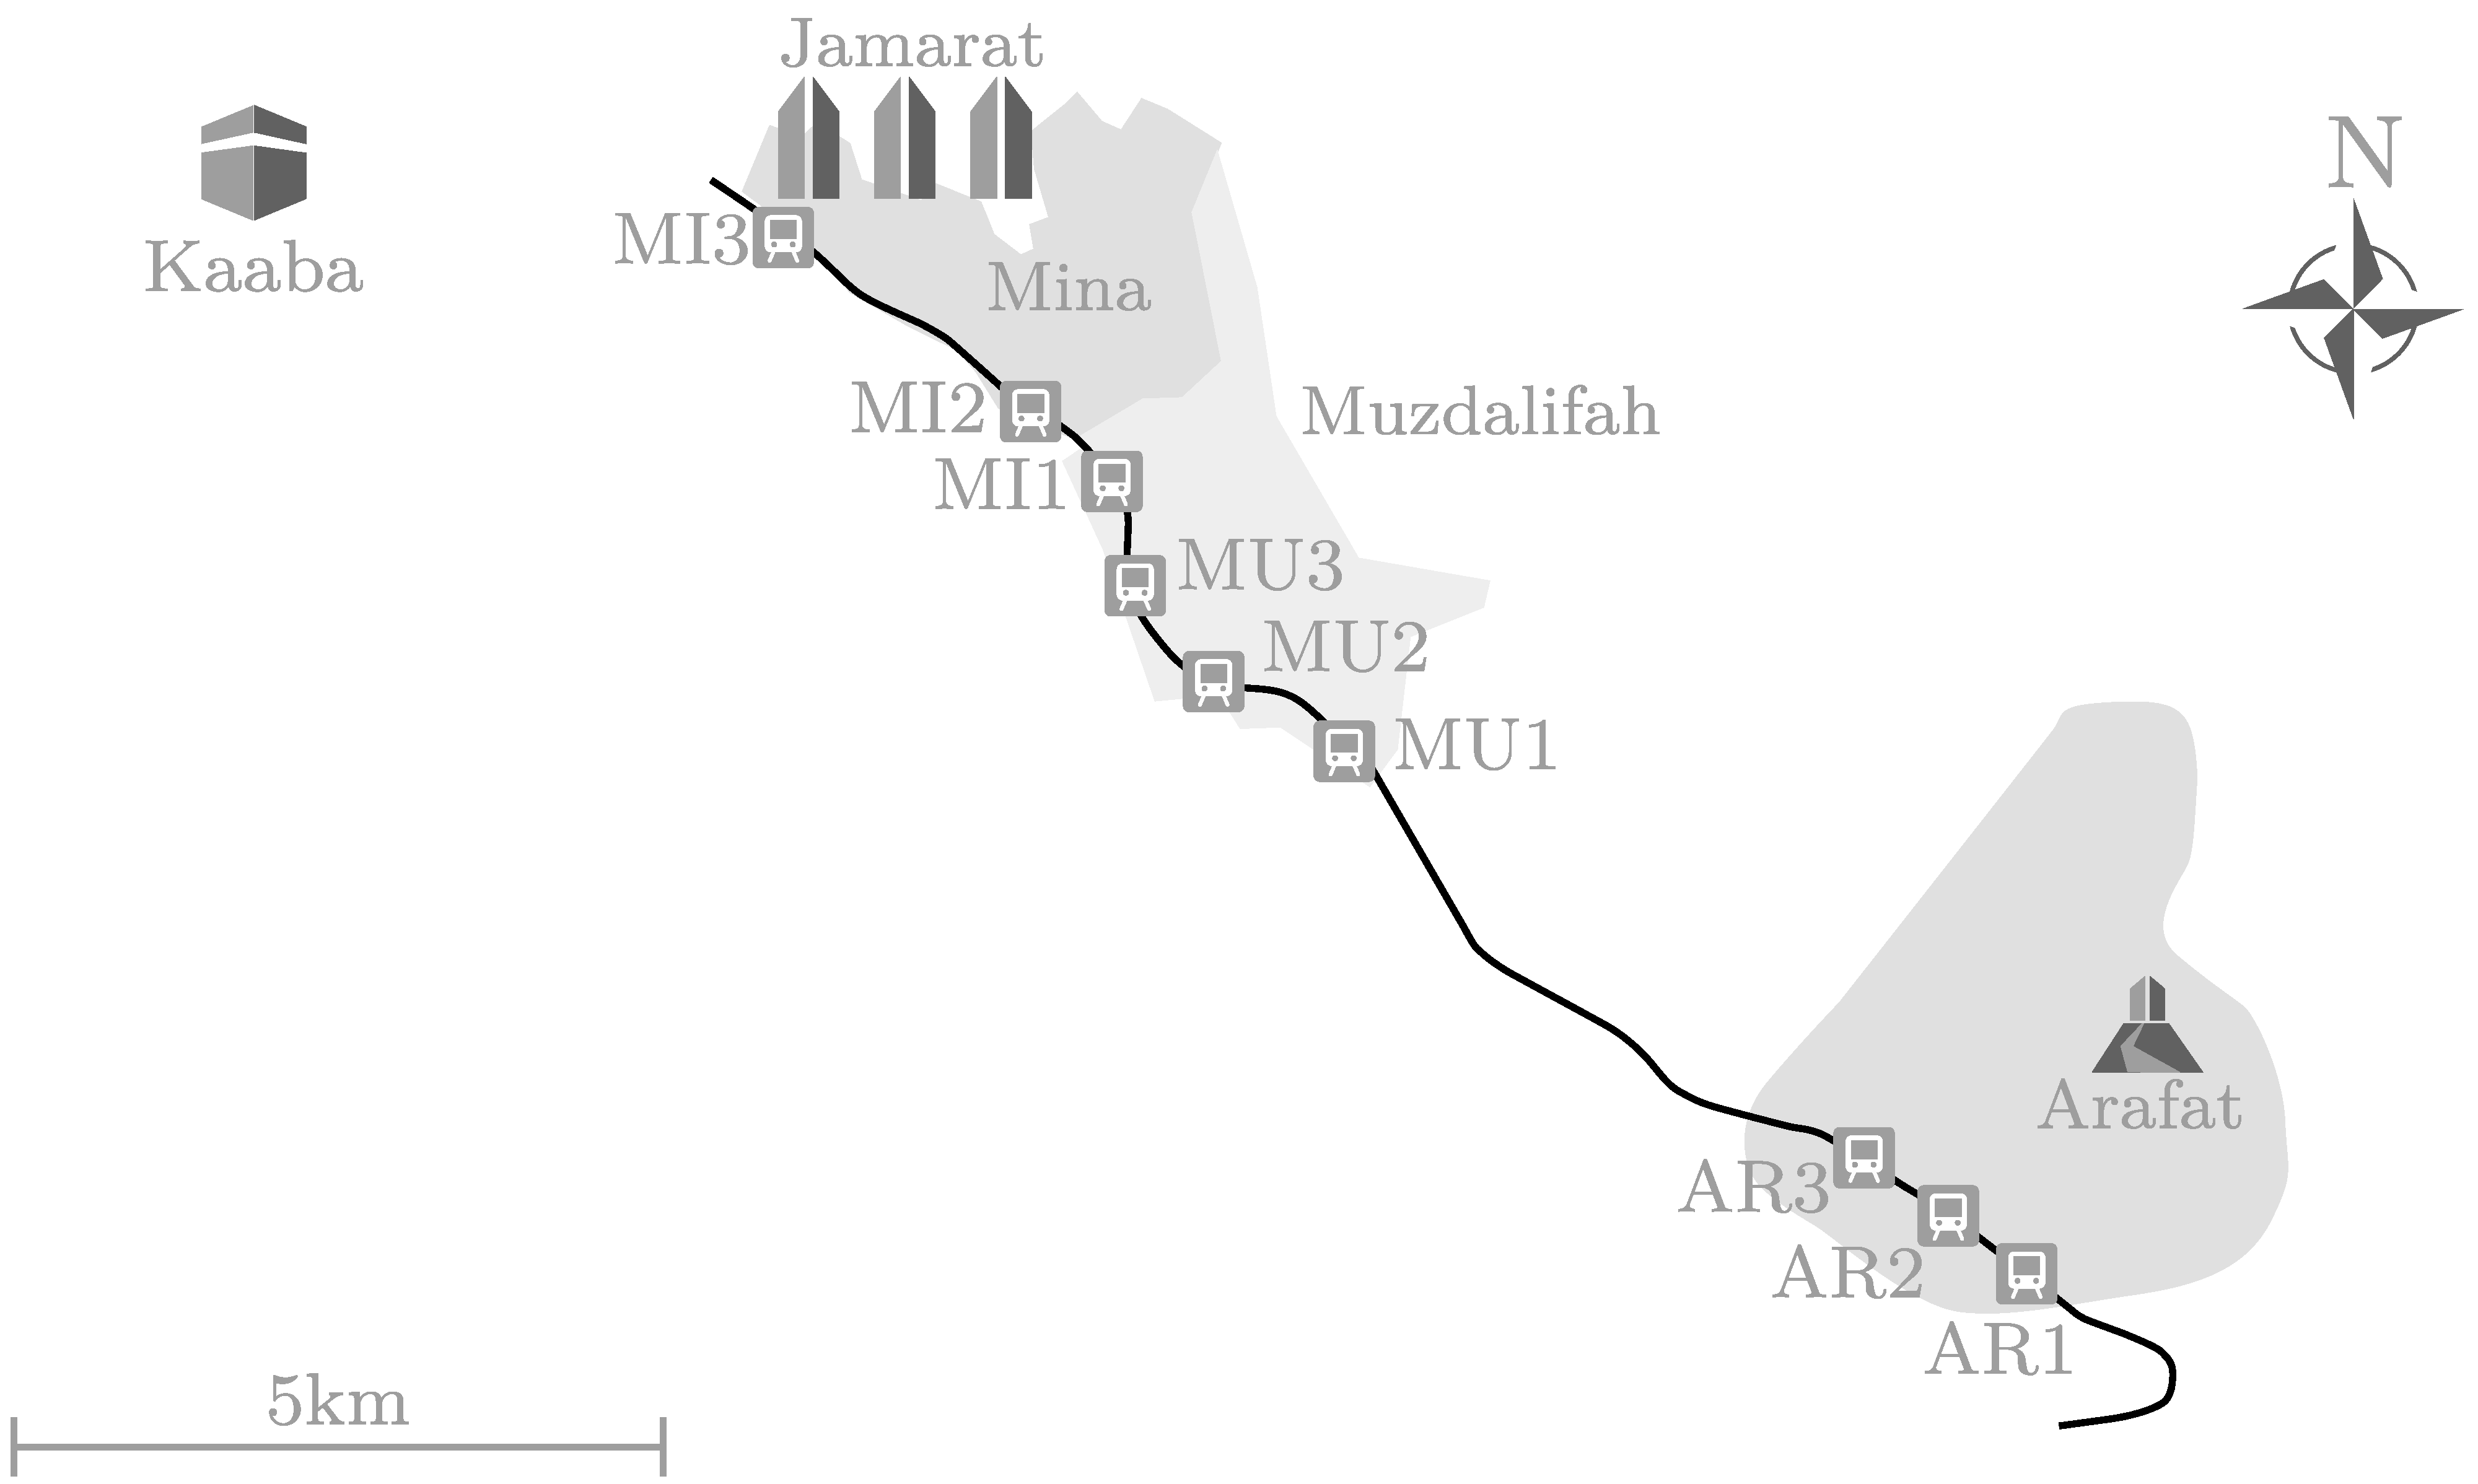
\includegraphics[width=0.8\textwidth]{images/Image.pdf}
	\caption{Schematische Abbildung der Metro in Mekka, Saudi Arabien.}
	\label{fig:food}
\end{figure}

\section{Literatur}
Quellen für Aussagen können in Klammern am Ende des Satzes stehen \parencite{kohlmorgen1999experiences}.
Alternativ kann auf eine Quelle ohne Klammern verwiesen werden, wie es z.B. in \textcite{haase2001beschaffungs} steht.

\section{Modell}
Hier führen wir unser Modell ein. Dazu unterteilen wir den Abschnitt in zwei Unterabschnitte. Achten Sie immer darauf, dass jeder Abschnitt oder Unterabschnitt mindestens eine Seite lang sein sollte. Ist das nicht der Fall, fassen Sie die Abschnitte lieber zusammen.

\subsection{Annahmen}
Die Modellierung des Sachverhaltes erfordert einige Abstraktionen. Die könnten Sie beispielsweise hier erläutern.

\subsection{Aufbau}
Mengen haben kalligraphische Symbole wie z.B. $\mathcal{J}$.
Für Variablen werden Großbuchstaben verwendet $X_j$, $j \in \mathcal{J}$, wobei für Parameter und Indizes Kleinbuchstaben verwendet werden $b_i$.
Das Modell ist wie folgt definiert:
\begin{align}
	\text{maximiere} \ F = & \sum_{j\in \mathcal{J}} c_j \times X_j\\
	\intertext{unter den Nebenbedingungen}
	& \sum_{j\in \mathcal{J}}a_{ij} \times X_j \leq b_i && \forall i\in \mathcal{I}\\
	\label{eq:nichtnegativitaet}
	&X_j \geq 0 && \forall j\in \mathcal{J}
\end{align}
Die Nebenbedingung (\ref{eq:nichtnegativitaet}) stellt die Nichtnegativität sicher.
Erläutern Sie stets die Zielfunktion und die Restriktionen.

\section{Rechenstudie}
Tabelle \ref{tab:ergebnisse} zeigt die Werte der Merkmalsausprägungen der Alternativen A, B und C.
\begin{table}[H]
	\centering
	\caption{Tabellen haben Überschriften}
	\label{tab:ergebnisse}
	\begin{tabular}{ccc}
		\toprule
		A & B & C\\
		\midrule
		1 & 2 & 3\\
		4 & 5 & 6 \\
		\bottomrule
	\end{tabular}
\end{table}

\section{Zusammenfassung und Ausblick}
Hier steht eine kurze Zusammenfassung und ein Ausblick auf sinnvolle Forschungsfragen, die aufbauend auf diese Arbeit durchgeführt werden können.

% Literaturverzeichnis ausgeben
\newpage
\pagenumbering{Roman}
\setcounter{page}{6}
\addcontentsline{toc}{section}{Literatur}
\printbibliography

\newpage
\section*{Eidesstattliche Erklärung}
Ich versichere an Eides statt, dass ich die vorstehende Arbeit selbstständig und ohne fremde Hilfe angefertigt und mich anderer als der im beigefügten Verzeichnis angegebenen Hilfsmittel nicht bedient habe. Alle Stellen, die wörtlich oder sinngemäß aus Veröffentlichungen übernommen wurden, sind als solche kenntlich gemacht. Alle Internetquellen sind der Arbeit beigefügt. Des Weiteren versichere ich, dass ich die Arbeit vorher nicht in einem anderen Prüfungsverfahren eingereicht habe und dass die eingereichte schriftliche Fassung der auf dem elektronischen Speichermedium entspricht.

\vspace{2cm}
\begin{flushleft}
Hamburg, Datum \\
\vspace{0.5cm}
Vorname Nachname \end{flushleft}
\end{document}
